\documentclass{article}
\usepackage{graphicx} % Required for inserting images
\usepackage[margin=1.0in]{geometry}
\usepackage{amsmath}
\usepackage{float}
\usepackage{hyperref}
\usepackage{listings}

\linespread{1}
\setlength{\parindent}{0pt} % Disable paragraph indentation

\title{CPEN 333 Final Project : Part I Alternative (Multithreaded Game)}
\author{Group G6 : Muntakim Rahman and Tomaz Zlindra}
\date{December 6th, 2024}

\begin{document}

\maketitle

\section{Redesign}
Our main redesign of the program structure was to change the model of Inter-Process Communication (IPC) from message passing to shared-memory.
This task was reduced to \texttt{producer-consumer} problems for each resource, in which the \texttt{producer} must wait for the \texttt{consumer} to yield the resource and vice-versa,
in order for the program to be thread-safe. \\

Having removed the use of the \texttt{Queue}, \texttt{QueueHandler} classes, we aimed to achieve synchronization with \texttt{semaphores} for
the \textit{4} shared resources (i.e. "\texttt{game\_over}", "\texttt{score}", "\texttt{prey}", "\texttt{move}") to indicate when they have been produced.
All, except for \texttt{"game\_over"} are protected via critical section using a \texttt{dict} of \texttt{mutexes}. \\

Please see the comment at the top of the \texttt{part1\_alternative.py} file for a description of the implementation. This file will describe the benefits, disadvantages, and challenges of this.

\section{Benefits}

Since we were able to eliminate the need for \textit{2} classes, this simplified the relationships between classes, as shown in Figure \ref{fig:Part1_Alternative_ClassDiagrams}. \\

\begin{figure}[H]
    \centering
    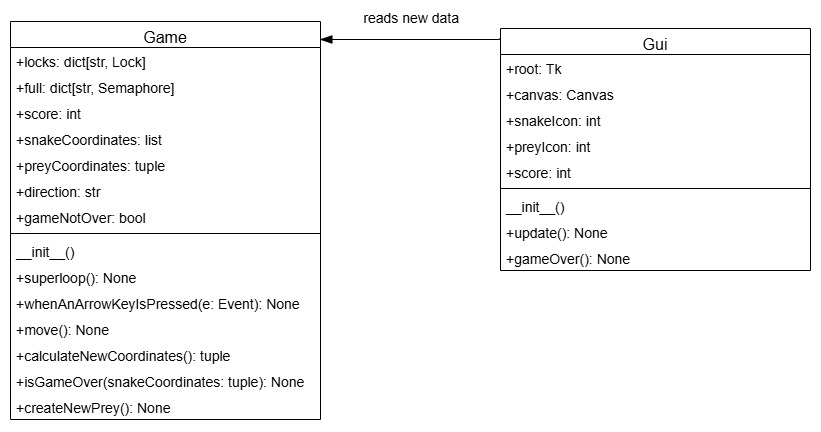
\includegraphics[width=0.7\textwidth]{../Part_1_Alternative_ClassDiagrams.jpg}
    \caption{Part 1 Alternative - UML Relationship}
    \label{fig:Part1_Alternative_ClassDiagrams}
\end{figure}

\subsection{Reader-Writer Abstraction}
If we abstract this to be a \texttt{reader-writer} synchronization problem, a single writer / many readers can access access the resource at all times.
We need to ensure there isn't a race condition between them. This is a problem we have addressed before (e.g. Lab 5). \\

We have designed this program to have the following constraints:

\begin{itemize}
    \item $\{ \text{Readers} \} \cup \{ 0, 1 \} \hspace{5px} \text{where} \hspace{5px} \{ \text{Writers} \} \cup \{ 0 \}$
    \item $\{ \text{Writers} \} \cup \{ 0, 1 \} \hspace{5px} \text{where} \hspace{5px} \{ \text{Readers} \} \cup \{ 0 \}$
    \item $\{ \text{Readers} \} \cup \{ 0 \} \hspace{5px} \text{where} \hspace{5px} \{ \text{Writers} \} \cup \{ 1 \}$
\end{itemize}

\subsubsection{Producer Behaviour}

The \texttt{game} instance acts as both a reader and a writer in different places. It reads the current value(s) of the shared resource and copies it for processing. It also writes the new data to the shared resource.
When it is behaving as a \texttt{reader}, we don't need to acquire the \texttt{mutex} or release the \texttt{semaphore}. Race conditions become a possibility for cases where the shared resources are being modified.

\section{Disadvantages}


\subsection{Additional Complexity}

We have to ensure that each of the shared resources are accessed effectively. More locks means that there are more critical sections to manage among threads.
We needed to ensure that critical sections were kept short and to the point to be able to navigate this added complexity. \\

In addition, we have the \texttt{full} semaphores to indicate when a new value is available. This condition must be evaluated by the \texttt{consumer} once it successfully acquires a \texttt{mutex}.

\subsection{Storage}

Along with the \texttt{mutexes} and \texttt{semaphores}, we also need to store the \texttt{game.preyCoordinates} data field for the \texttt{gui} instance. This wasn't necessary with the \texttt{queue} implementation.

\section{Challenges}

We initially spawned two threads for the \texttt{game.superloop()} and \texttt{gui.update()} methods.
This was highly problematic since the program functioned as intended for initial gameplay. Critical sections seemed to be thread-safe, both theoretically and in practice.
However, through extensive testing we observed this consistently caused the program to crash when the snake grew at a score $\sim$ \textit{25-26}. \\

We realized why the original program design had the \texttt{QueueHandler.queueHandler()} method schedule itself with the \texttt{Tk.after(100)} method.
From referring to the \texttt{Python} documentation, we realized that \texttt{Tkinter} widget updates must be done by the main thread. \\

\textit{(See The Python Software Foundation. (n.d.). Tkinter - Python interface to TCL/TK. Python Documentation. \href{https://docs.python.org/3/library/tkinter.html\#threading-model}{https://docs.python.org/3/library/tkinter.html\#threading-model})}

\subsection{Solution}

Instead of having the \texttt{gui.update()} method execute loop with spinlocks, we wrote it to be a conditional statement which schedules itself using the \texttt{Tk.after(100)} method.
We implemented this with non-blocking acquires as well, such that the inability to enter a critical section wouldn't block other widget updates from occuring in the meantime.

\end{document}
